\documentclass{beamer}
\addtobeamertemplate{navigation symbols}{}{%
\usebeamerfont{footline}%
\usebeamercolor[fg]{footline}%
\hspace{5em}%
Слайд №\insertframenumber
}
\setbeamercolor{footline}{fg=blue}
%\usetheme{Warsaw}

\usepackage[english, russian]{babel}

\usepackage{fontspec}
\setmainfont{Times New Roman}
\setsansfont{Times New Roman}
\setmonofont{Consolas}

\usepackage{sudoku}
\usepackage{tikz}
\usepackage[cache=false]{minted}
\newminted{python}{fontsize=\scriptsize, linenos=false}

\graphicspath{{../images/}}

\title{Решатель судоку по изображению с камеры}
\subtitle{}
\author{А.~А.~Муравцев\inst{1}}

\institute{
\inst{1}
Высшая школа теоретической механики\\
Санкт-Петербургский Политехнический университет Петра Великого
}


\begin{document}

\renewcommand*\sudokuformat[1]{\Large\sffamily#1}

\frame{\titlepage}

\begin{frame}
\frametitle{Структура проекта}
\tableofcontents
\end{frame}

\section{Обработка изображения и распознавание}

\subsection{Общая обработка полученного изображения}

\subsection{Определение положения поля судоку на обработанном изображении}

\subsection{Разделение на ячейки}

\section{Решатель судоку}


\begin{frame}
\frametitle{Распознавание поля судоку}

\begin{center}
\setlength\sudokusize{6cm}
\begin{sudoku-block}
| |2| | |3| |9| |7|.
| |1| | | | | | | |.
|4| |7| | | |2| |8|.
| | |5|2| | | |9| |.
| | | |1|8| |7| | |.
| |4| | | |3| | | |.
| | | | |6| | |7|1|.
| |7| | | | | | | |.
|9| |3| |2| |6| |5|.
\end{sudoku-block}
\end{center}

\end{frame}


\begin{frame}
\frametitle{Разделение на ячейки}
\end{frame}


\begin{frame}
\frametitle{Преобразование в чёрно-белое изображение}
\begin{center}
\begin{tikzpicture}
	\node[inner sep=0pt] (to_black_white) at (0,0) {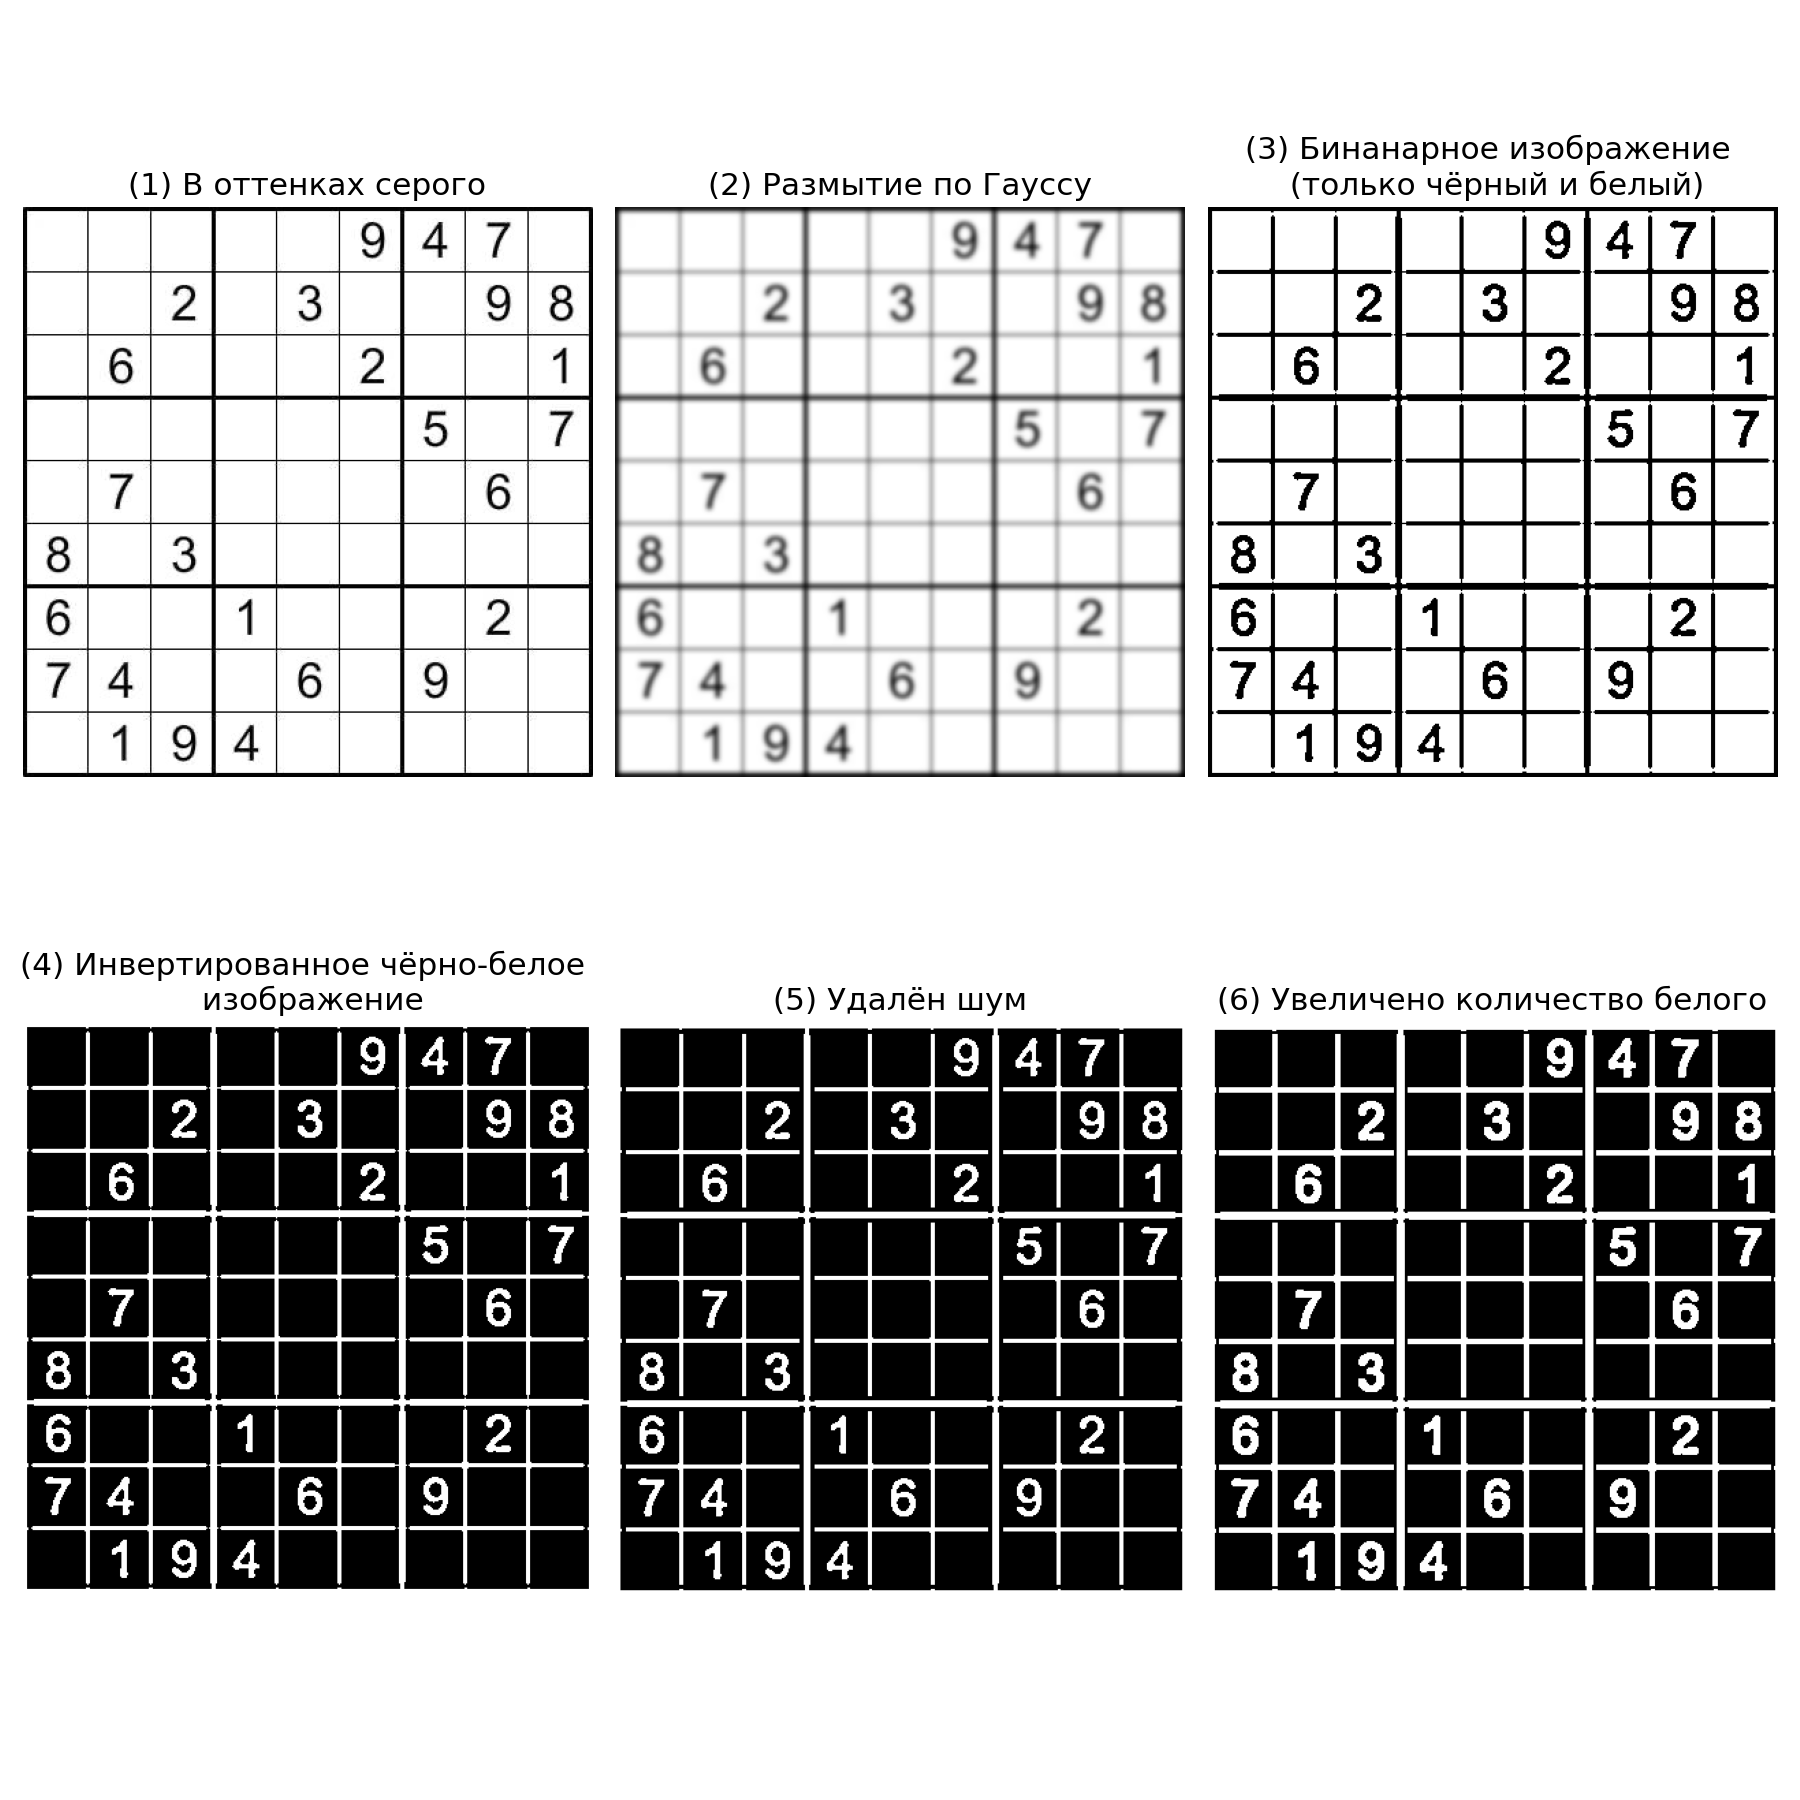
\includegraphics[width=0.7\textwidth]{to_black_white}};
\end{tikzpicture}
\end{center}

\end{frame}


\section{Графическое приложение на PyQT}

\begin{frame}
\frametitle{Интерфейс GUI-приложения}
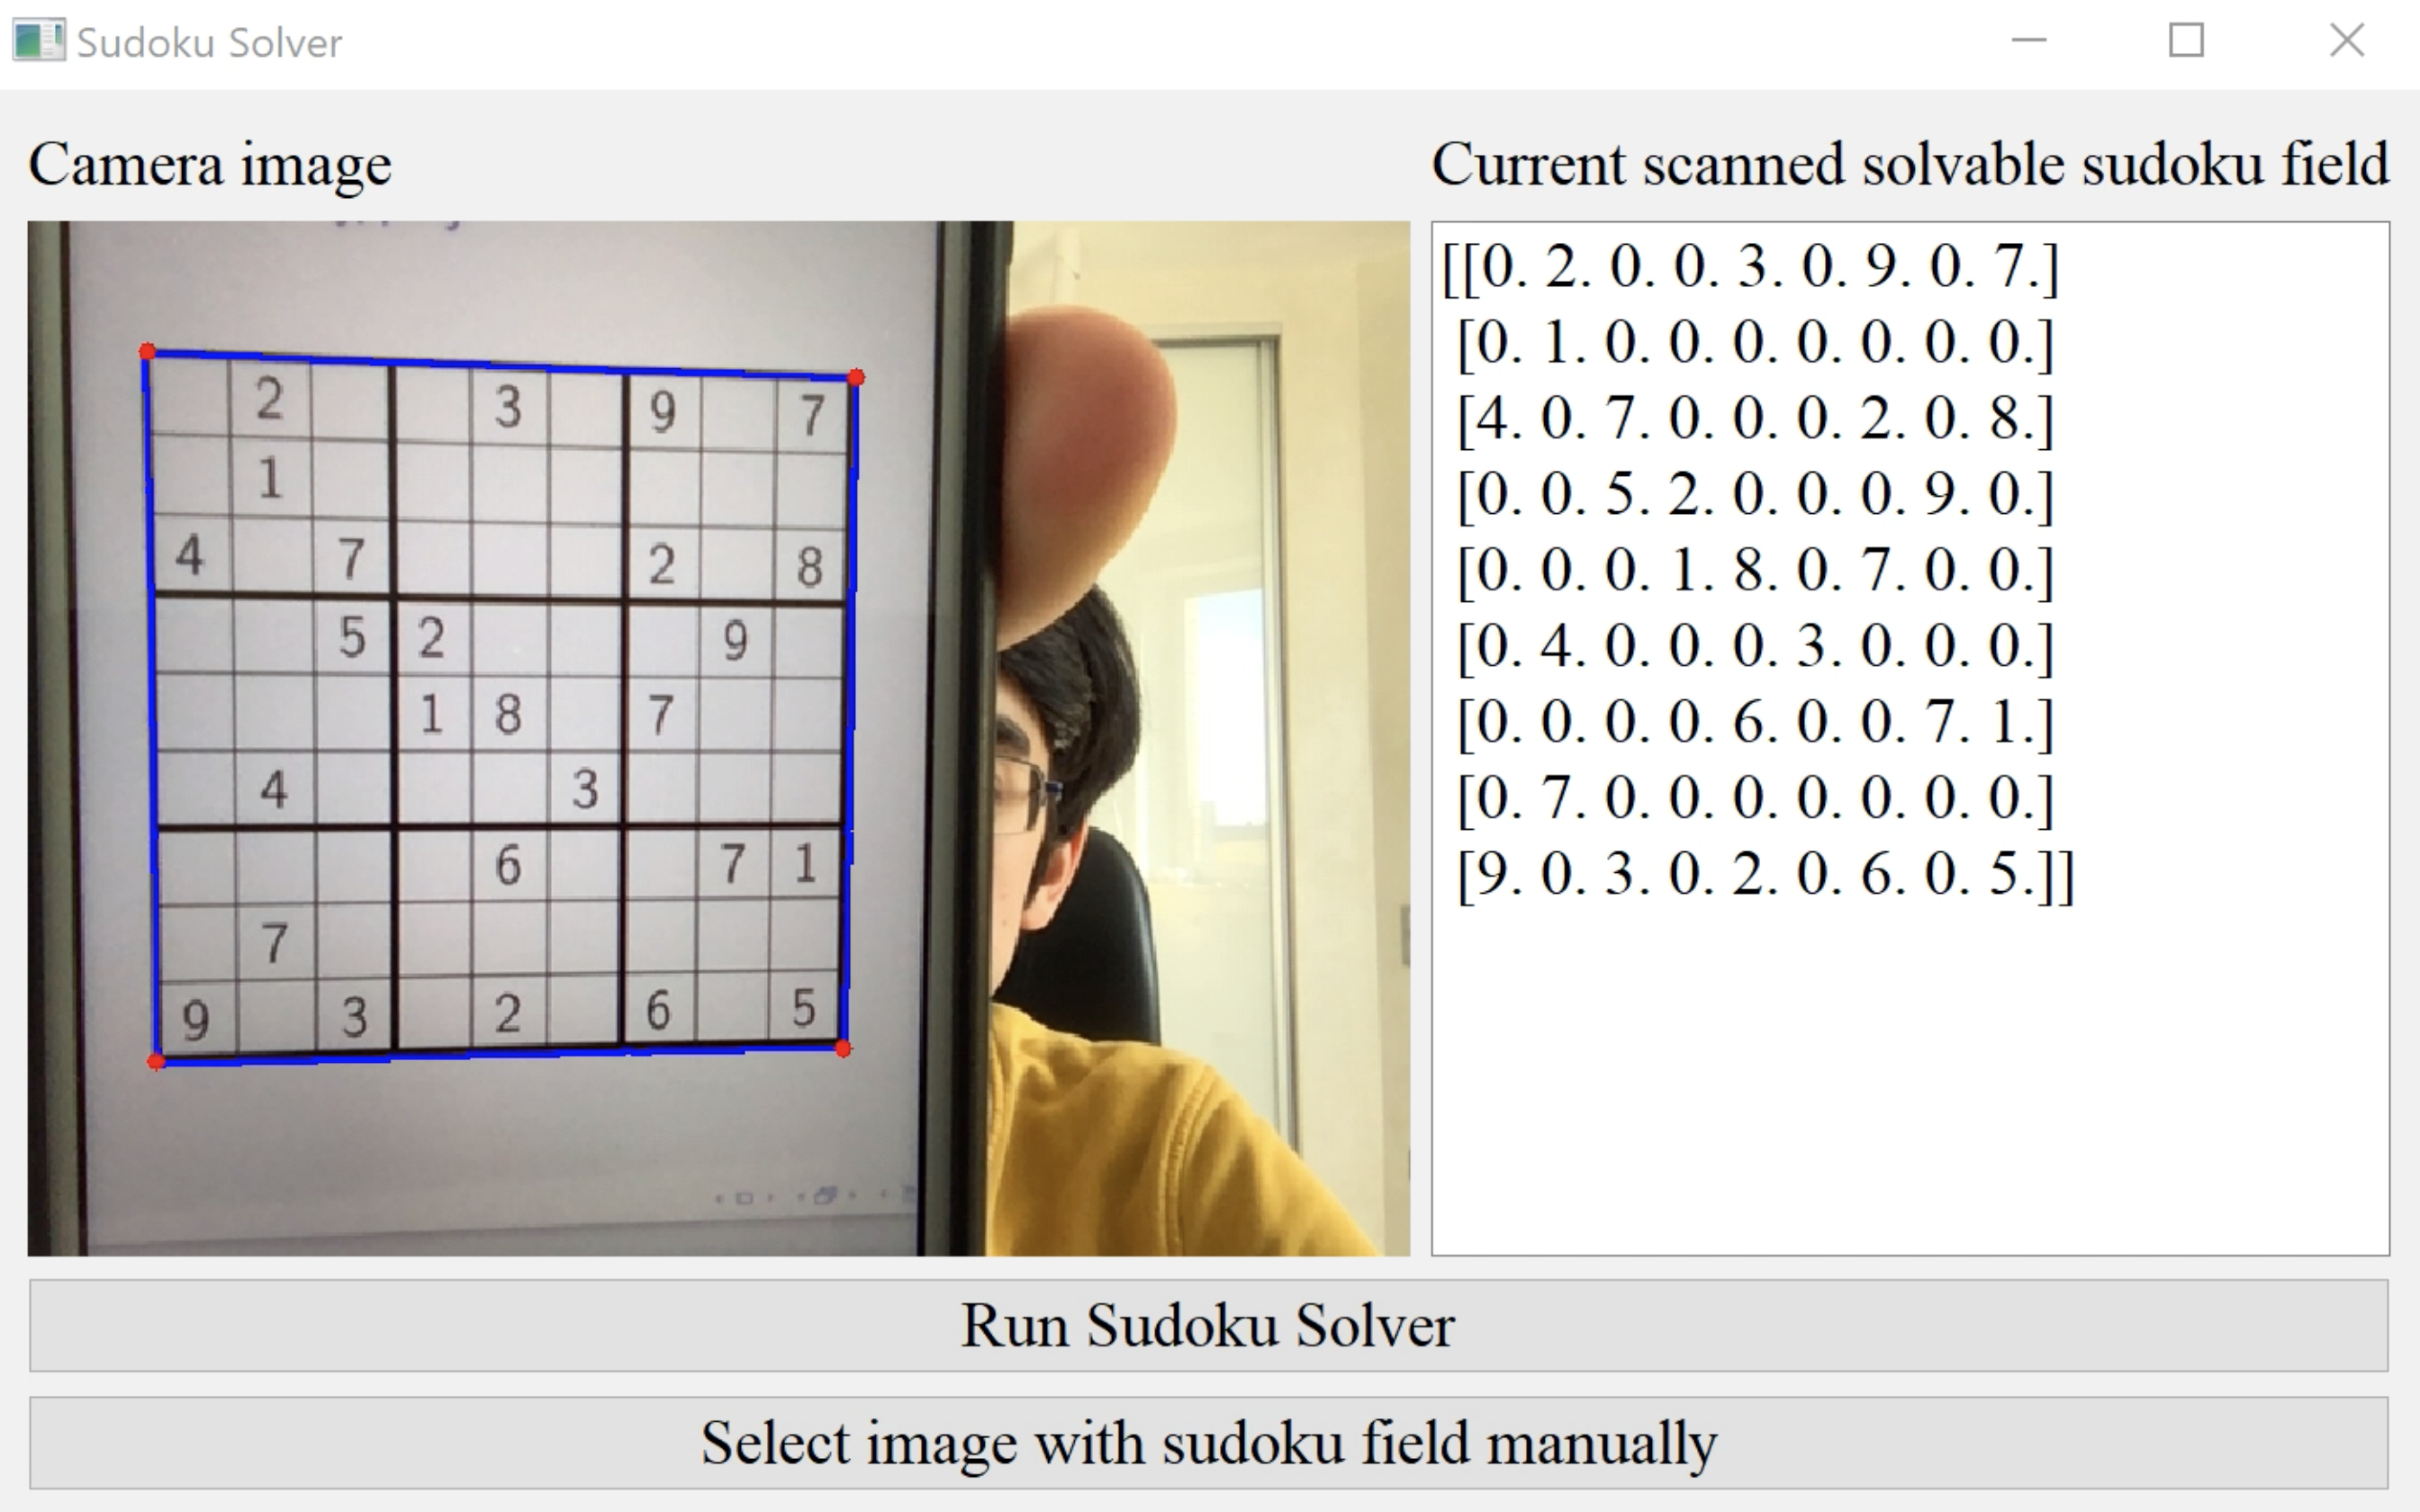
\includegraphics[width=\textwidth]{sudoku_app_in_action}
\end{frame}



\begin{frame}[fragile]
\frametitle{Слоты PyQT}

Слот преобразования openCV изображения в PyQT изображение:
\begin{pythoncode}
    @pyqtSlot(np.ndarray)
    def update_image(self, cv_img):
        """Updates the image_label with a new openCV image"""
        qt_img = self.convert_cv_to_qt(cv_img)
        self.frame_field.setPixmap(qt_img)
\end{pythoncode}
\ \\
Слот обновления текста внутри QTextEdit:
\begin{pythoncode}
    @pyqtSlot(np.ndarray)
    def update_text(self, sudoku_to_solve):
        """Updates the image_label with a new openCV image"""
        self.scanned_sudoku.setText(np.array2string(sudoku_to_solve))
\end{pythoncode}

\end{frame}


\begin{frame}[fragile]
\frametitle{Поток с результатом}
\begin{pythoncode}
class ThreadWithResult(threading.Thread):
    def __init__(self, group=None, target=None, name=None,
                 args=(), kwargs={}, *, daemon=None):
        self.result = None

        def function():
            self.result = target(*args, **kwargs)
        super().__init__(group=group, target=function,
                         name=name, daemon=daemon)
\end{pythoncode}

\end{frame}
\end{document}
